% Options for packages loaded elsewhere
\PassOptionsToPackage{unicode}{hyperref}
\PassOptionsToPackage{hyphens}{url}
\PassOptionsToPackage{dvipsnames,svgnames,x11names}{xcolor}
%
\documentclass[
  a4paper,
  DIV=11,
  numbers=noendperiod,
  onepage,
  openany]{scrreprt}

\usepackage{amsmath,amssymb}
\usepackage{iftex}
\ifPDFTeX
  \usepackage[T1]{fontenc}
  \usepackage[utf8]{inputenc}
  \usepackage{textcomp} % provide euro and other symbols
\else % if luatex or xetex
  \usepackage{unicode-math}
  \defaultfontfeatures{Scale=MatchLowercase}
  \defaultfontfeatures[\rmfamily]{Ligatures=TeX,Scale=1}
\fi
\usepackage{lmodern}
\ifPDFTeX\else  
    % xetex/luatex font selection
\fi
% Use upquote if available, for straight quotes in verbatim environments
\IfFileExists{upquote.sty}{\usepackage{upquote}}{}
\IfFileExists{microtype.sty}{% use microtype if available
  \usepackage[]{microtype}
  \UseMicrotypeSet[protrusion]{basicmath} % disable protrusion for tt fonts
}{}
\makeatletter
\@ifundefined{KOMAClassName}{% if non-KOMA class
  \IfFileExists{parskip.sty}{%
    \usepackage{parskip}
  }{% else
    \setlength{\parindent}{0pt}
    \setlength{\parskip}{6pt plus 2pt minus 1pt}}
}{% if KOMA class
  \KOMAoptions{parskip=half}}
\makeatother
\usepackage{xcolor}
\usepackage[lmargin=30mm,rmargin=30mm,tmargin=35mm,bmargin=30mm]{geometry}
\setlength{\emergencystretch}{3em} % prevent overfull lines
\setcounter{secnumdepth}{5}
% Make \paragraph and \subparagraph free-standing
\makeatletter
\ifx\paragraph\undefined\else
  \let\oldparagraph\paragraph
  \renewcommand{\paragraph}{
    \@ifstar
      \xxxParagraphStar
      \xxxParagraphNoStar
  }
  \newcommand{\xxxParagraphStar}[1]{\oldparagraph*{#1}\mbox{}}
  \newcommand{\xxxParagraphNoStar}[1]{\oldparagraph{#1}\mbox{}}
\fi
\ifx\subparagraph\undefined\else
  \let\oldsubparagraph\subparagraph
  \renewcommand{\subparagraph}{
    \@ifstar
      \xxxSubParagraphStar
      \xxxSubParagraphNoStar
  }
  \newcommand{\xxxSubParagraphStar}[1]{\oldsubparagraph*{#1}\mbox{}}
  \newcommand{\xxxSubParagraphNoStar}[1]{\oldsubparagraph{#1}\mbox{}}
\fi
\makeatother

\usepackage{color}
\usepackage{fancyvrb}
\newcommand{\VerbBar}{|}
\newcommand{\VERB}{\Verb[commandchars=\\\{\}]}
\DefineVerbatimEnvironment{Highlighting}{Verbatim}{commandchars=\\\{\}}
% Add ',fontsize=\small' for more characters per line
\usepackage{framed}
\definecolor{shadecolor}{RGB}{241,243,245}
\newenvironment{Shaded}{\begin{snugshade}}{\end{snugshade}}
\newcommand{\AlertTok}[1]{\textcolor[rgb]{0.68,0.00,0.00}{#1}}
\newcommand{\AnnotationTok}[1]{\textcolor[rgb]{0.37,0.37,0.37}{#1}}
\newcommand{\AttributeTok}[1]{\textcolor[rgb]{0.40,0.45,0.13}{#1}}
\newcommand{\BaseNTok}[1]{\textcolor[rgb]{0.68,0.00,0.00}{#1}}
\newcommand{\BuiltInTok}[1]{\textcolor[rgb]{0.00,0.23,0.31}{#1}}
\newcommand{\CharTok}[1]{\textcolor[rgb]{0.13,0.47,0.30}{#1}}
\newcommand{\CommentTok}[1]{\textcolor[rgb]{0.37,0.37,0.37}{#1}}
\newcommand{\CommentVarTok}[1]{\textcolor[rgb]{0.37,0.37,0.37}{\textit{#1}}}
\newcommand{\ConstantTok}[1]{\textcolor[rgb]{0.56,0.35,0.01}{#1}}
\newcommand{\ControlFlowTok}[1]{\textcolor[rgb]{0.00,0.23,0.31}{\textbf{#1}}}
\newcommand{\DataTypeTok}[1]{\textcolor[rgb]{0.68,0.00,0.00}{#1}}
\newcommand{\DecValTok}[1]{\textcolor[rgb]{0.68,0.00,0.00}{#1}}
\newcommand{\DocumentationTok}[1]{\textcolor[rgb]{0.37,0.37,0.37}{\textit{#1}}}
\newcommand{\ErrorTok}[1]{\textcolor[rgb]{0.68,0.00,0.00}{#1}}
\newcommand{\ExtensionTok}[1]{\textcolor[rgb]{0.00,0.23,0.31}{#1}}
\newcommand{\FloatTok}[1]{\textcolor[rgb]{0.68,0.00,0.00}{#1}}
\newcommand{\FunctionTok}[1]{\textcolor[rgb]{0.28,0.35,0.67}{#1}}
\newcommand{\ImportTok}[1]{\textcolor[rgb]{0.00,0.46,0.62}{#1}}
\newcommand{\InformationTok}[1]{\textcolor[rgb]{0.37,0.37,0.37}{#1}}
\newcommand{\KeywordTok}[1]{\textcolor[rgb]{0.00,0.23,0.31}{\textbf{#1}}}
\newcommand{\NormalTok}[1]{\textcolor[rgb]{0.00,0.23,0.31}{#1}}
\newcommand{\OperatorTok}[1]{\textcolor[rgb]{0.37,0.37,0.37}{#1}}
\newcommand{\OtherTok}[1]{\textcolor[rgb]{0.00,0.23,0.31}{#1}}
\newcommand{\PreprocessorTok}[1]{\textcolor[rgb]{0.68,0.00,0.00}{#1}}
\newcommand{\RegionMarkerTok}[1]{\textcolor[rgb]{0.00,0.23,0.31}{#1}}
\newcommand{\SpecialCharTok}[1]{\textcolor[rgb]{0.37,0.37,0.37}{#1}}
\newcommand{\SpecialStringTok}[1]{\textcolor[rgb]{0.13,0.47,0.30}{#1}}
\newcommand{\StringTok}[1]{\textcolor[rgb]{0.13,0.47,0.30}{#1}}
\newcommand{\VariableTok}[1]{\textcolor[rgb]{0.07,0.07,0.07}{#1}}
\newcommand{\VerbatimStringTok}[1]{\textcolor[rgb]{0.13,0.47,0.30}{#1}}
\newcommand{\WarningTok}[1]{\textcolor[rgb]{0.37,0.37,0.37}{\textit{#1}}}

\providecommand{\tightlist}{%
  \setlength{\itemsep}{0pt}\setlength{\parskip}{0pt}}\usepackage{longtable,booktabs,array}
\usepackage{calc} % for calculating minipage widths
% Correct order of tables after \paragraph or \subparagraph
\usepackage{etoolbox}
\makeatletter
\patchcmd\longtable{\par}{\if@noskipsec\mbox{}\fi\par}{}{}
\makeatother
% Allow footnotes in longtable head/foot
\IfFileExists{footnotehyper.sty}{\usepackage{footnotehyper}}{\usepackage{footnote}}
\makesavenoteenv{longtable}
\usepackage{graphicx}
\makeatletter
\def\maxwidth{\ifdim\Gin@nat@width>\linewidth\linewidth\else\Gin@nat@width\fi}
\def\maxheight{\ifdim\Gin@nat@height>\textheight\textheight\else\Gin@nat@height\fi}
\makeatother
% Scale images if necessary, so that they will not overflow the page
% margins by default, and it is still possible to overwrite the defaults
% using explicit options in \includegraphics[width, height, ...]{}
\setkeys{Gin}{width=\maxwidth,height=\maxheight,keepaspectratio}
% Set default figure placement to htbp
\makeatletter
\def\fps@figure{htbp}
\makeatother

\KOMAoption{captions}{tableheading}
\makeatletter
\@ifpackageloaded{tcolorbox}{}{\usepackage[skins,breakable]{tcolorbox}}
\@ifpackageloaded{fontawesome5}{}{\usepackage{fontawesome5}}
\definecolor{quarto-callout-color}{HTML}{909090}
\definecolor{quarto-callout-note-color}{HTML}{0758E5}
\definecolor{quarto-callout-important-color}{HTML}{CC1914}
\definecolor{quarto-callout-warning-color}{HTML}{EB9113}
\definecolor{quarto-callout-tip-color}{HTML}{00A047}
\definecolor{quarto-callout-caution-color}{HTML}{FC5300}
\definecolor{quarto-callout-color-frame}{HTML}{acacac}
\definecolor{quarto-callout-note-color-frame}{HTML}{4582ec}
\definecolor{quarto-callout-important-color-frame}{HTML}{d9534f}
\definecolor{quarto-callout-warning-color-frame}{HTML}{f0ad4e}
\definecolor{quarto-callout-tip-color-frame}{HTML}{02b875}
\definecolor{quarto-callout-caution-color-frame}{HTML}{fd7e14}
\makeatother
\makeatletter
\@ifpackageloaded{bookmark}{}{\usepackage{bookmark}}
\makeatother
\makeatletter
\@ifpackageloaded{caption}{}{\usepackage{caption}}
\AtBeginDocument{%
\ifdefined\contentsname
  \renewcommand*\contentsname{Table of contents}
\else
  \newcommand\contentsname{Table of contents}
\fi
\ifdefined\listfigurename
  \renewcommand*\listfigurename{List of Figures}
\else
  \newcommand\listfigurename{List of Figures}
\fi
\ifdefined\listtablename
  \renewcommand*\listtablename{List of Tables}
\else
  \newcommand\listtablename{List of Tables}
\fi
\ifdefined\figurename
  \renewcommand*\figurename{Figure}
\else
  \newcommand\figurename{Figure}
\fi
\ifdefined\tablename
  \renewcommand*\tablename{Table}
\else
  \newcommand\tablename{Table}
\fi
}
\@ifpackageloaded{float}{}{\usepackage{float}}
\floatstyle{ruled}
\@ifundefined{c@chapter}{\newfloat{codelisting}{h}{lop}}{\newfloat{codelisting}{h}{lop}[chapter]}
\floatname{codelisting}{Listing}
\newcommand*\listoflistings{\listof{codelisting}{List of Listings}}
\makeatother
\makeatletter
\makeatother
\makeatletter
\@ifpackageloaded{caption}{}{\usepackage{caption}}
\@ifpackageloaded{subcaption}{}{\usepackage{subcaption}}
\makeatother

\ifLuaTeX
  \usepackage{selnolig}  % disable illegal ligatures
\fi
\usepackage{bookmark}

\IfFileExists{xurl.sty}{\usepackage{xurl}}{} % add URL line breaks if available
\urlstyle{same} % disable monospaced font for URLs
\hypersetup{
  pdftitle={Tutorial de Django Girls},
  pdfauthor={Lcdo. Diego Medardo Saavedra García, Mgtr.},
  colorlinks=true,
  linkcolor={blue},
  filecolor={Maroon},
  citecolor={Blue},
  urlcolor={Blue},
  pdfcreator={LaTeX via pandoc}}


\title{Tutorial de Django Girls}
\author{Lcdo. Diego Medardo Saavedra García, Mgtr.}
\date{Jul 11, 2024}

\begin{document}
\maketitle

\renewcommand*\contentsname{Table of contents}
{
\hypersetup{linkcolor=}
\setcounter{tocdepth}{2}
\tableofcontents
}

\bookmarksetup{startatroot}

\chapter{Bienvenido}\label{bienvenido}

Bienvenida al libro

Descripción del Curso general \#\# ¿De qué trata este curso?

En esta sección describimos de que va a tratar el curso \#\# ¿Para quién
es este curso?

En esta sección mencionamos el público objetivo \#\# ¿Cómo contribuir?

En esta sección describimos como se puede contribuir al libro

\part{Introducción}

\chapter{Tutorial de Django Girls}\label{tutorial-de-django-girls}

\begin{tcolorbox}[enhanced jigsaw, colbacktitle=quarto-callout-tip-color!10!white, colback=white, breakable, bottomrule=.15mm, opacityback=0, colframe=quarto-callout-tip-color-frame, toprule=.15mm, leftrule=.75mm, coltitle=black, bottomtitle=1mm, rightrule=.15mm, opacitybacktitle=0.6, toptitle=1mm, titlerule=0mm, left=2mm, arc=.35mm, title=\textcolor{quarto-callout-tip-color}{\faLightbulb}\hspace{0.5em}{Tip}]

Este trabajo está bajo la licencia internacional Creative Commons
Attribution-ShareAlike 4.0. Para ver una copia de esta licencia, visita
el siguiente enlace
\url{https://creativecommons.org/licenses/by-sa/4.0/}

\end{tcolorbox}

\chapter{Bienvenida/o}\label{bienvenidao}

¡Bienvenido/a al tutorial de las Django Girls! ¡Nos alegra que estés
aquí :) En este tutorial, te llevaremos de viaje a las entrañas de la
tecnología web, para que veas todas las piezas que se necesitan para que
la web funcione.

Como pasa con todas las cosas nuevas, va a ser una aventura - pero no te
preocupes; una vez que te has decidido a empezar, te irá de maravilla :)

\chapter{Introducción}\label{introducciuxf3n-1}

¿Alguna vez has tenido la sensación de que el mundo es cada vez más
tecnológico? ¿que cada vez lo entiendes menos? ¿Alguna vez te has
planteado crear un sitio web pero no sabías por dónde empezar? ¿Has
pensado alguna vez que el mundo del software es demasiado complicado
como para intentar hacer algo por tu cuenta?

Bueno, ¡tenemos buenas noticias! Programar no es tan difícil como parece
y queremos demostrarte lo divertido que puede llegar a ser.

Este tutorial no te convertirá en programadora de la noche a la mañana.
Si quieres ser buena en esto, necesitarás meses o incluso años de
aprendizaje y práctica. Sin embargo queremos enseñarte que programar o
crear sitios web no es tan complicado como parece. Intentaremos explicar
las cosas lo mejor que podamos, para perderle el miedo a la tecnología.

¡Esperamos conseguir que te guste la tecnología tanto como a nosotras!

\chapter{¿Qué aprenderás con este
tutorial?}\label{quuxe9-aprenderuxe1s-con-este-tutorial}

Cuando termines el tutorial, tendrás una aplicación web sencilla y
funcional: tu propio blog. Te mostraremos como ponerla en línea, ¡para
que otros puedan ver tu trabajo!

Tendrá (más o menos) esta pinta:

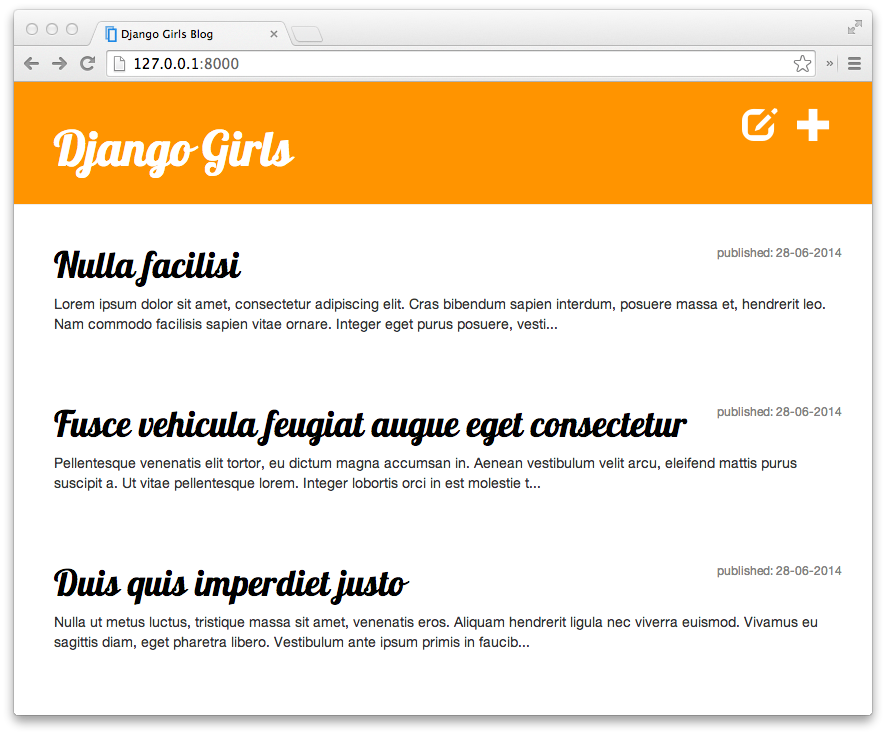
\includegraphics{unidades/unidad1/images/paste-2.png}

Bien, empecemos por el comienzo\ldots{}

\chapter{Seguir el tutorial desde
casa}\label{seguir-el-tutorial-desde-casa}

Participar en un taller de Django Girls en vivo es genial, pero somos
conscientes de que no siempre es posible hacerlo. Por eso, te
recomendamos hacer este tutorial en casa. Para las que estáis en casa,
estamos preparando vídeos que facilitarán seguir el tutorial por tu
cuenta. Todavía está en progreso, pero cada vez hay más cosas explicadas
en el canal de YouTube
\href{https://www.youtube.com/channel/UC0hNd2uW8jTR5K3KBzRuG2A/feed}{Coding
is for girls} (Nota: en inglés).

En cada capítulo hay un enlace que lleva al vídeo correspondiente (si lo
hay).

\chapter{Sobre nosotros y Cómo
contribuir}\label{sobre-nosotros-y-cuxf3mo-contribuir}

Este tutorial lo mantiene DjangoGirls. Si encuentras algún error o
quieres actualizar el tutorial, por favor sigue la guía de cómo
contribuir.

\chapter{¿Te gustaría ayudarnos a traducir el tutorial a otros
idiomas?}\label{te-gustaruxeda-ayudarnos-a-traducir-el-tutorial-a-otros-idiomas}

Actualmente, las traducciones se hacen en la plataforma crowdin.com, en
el siguiente enlace:

\url{https://crowdin.com/project/django-girls-tutorial}

Si tu idioma no aparece en la lista de crowdin, por favor abre un nuevo
issue con el idioma para que podamos añadirlo.

\part{Instalación}

\chapter{Si estás haciendo el tutorial en
casa}\label{si-estuxe1s-haciendo-el-tutorial-en-casa}

Si estás haciendo el tutorial en casa, y no en uno de los eventos de
Django Girls, puedes saltar este capítulo por completo e ir directamente
al capítulo ¿cómo funciona Internet?.

Esto es porque cubrimos las instalaciones de cosas a medida que se
requieran en el tutorial -- esta es solamente una página adicional que
reúne toda la información de instalación en un solo lugar (lo que es
útil para algunos formatos de taller). Puedes escoger instalar todo lo
que está en esta página ya mismo si lo deseas. Pero si quieres empezar a
aprender cosas antes de instalar un grupo de materiales en tu
computadora, salta este capítulo y te explicaremos las partes de la
instalación luego, cuando sean necesarias.

¡Buena suerte!

\chapter{Si estás asistiendo a un
workshop}\label{si-estuxe1s-asistiendo-a-un-workshop}

Si estás asistiendo a uno de los Django Girls events:

\begin{itemize}
\item
  Tu workshop puede tener una ``fiesta de instalación'' antes del
  workshop principal. Si estás en un equipo de instalación, ¡ésta página
  es para ti! Sigue las instrucciones aquí para obtener todo lo que tu
  necesitas para el workshop de instalación, con la ayuda de los
  entrenadores si lo necesitas. Entonces en el workshop principal, tu
  estarás preparado para saltar las instrucciones de instalación que
  encontrarás en el tutorial principal cuando llegues a ellos.
\item
  Los organizadores del taller pueden pedirte que en casa intentes
  instalar todo en tu computadora antes de iniciar el taller. Si has
  estado preguntando cómo hacer esto, ¡esta página es para ti! Sigue las
  instrucciones aquí, lo mejor puedas. Así, en el taller principal,
  cuando estés en uno de los pasos de la instalación del tutorial, y si
  no tenías esa pieza instalada, puedes pedir ayuda a una de tus
  entrenadoras.
\item
  Si tu taller no tiene una sesión de instalación (o no pudiste
  asistir), y si los organizadores no te piden que intentes instalar
  todo antes de tu llegada, salta esta página y ve al capítulo Cómo el
  internet funciona. Instalarás todo lo que necesitas para trabajar a lo
  largo del tutorial.
\end{itemize}

\chapter{Instalación}\label{instalaciuxf3n-1}

En este tutorial vas a construir un blog. Según cómo vayas a través del
tutorial, serás instruida en cómo instalar varios softwares en tu
computadora y configurar algunas cuentas online como sean necesarias.
Esta página reune todas las instalaciones e instrucciones del registro
en un lugar (el cual es útil para algunos formatos del taller).

\textbf{Si utilizas Chromebook, por favor sigue estas instrucciones.}

\begin{tcolorbox}[enhanced jigsaw, colbacktitle=quarto-callout-tip-color!10!white, colback=white, breakable, bottomrule=.15mm, opacityback=0, colframe=quarto-callout-tip-color-frame, toprule=.15mm, leftrule=.75mm, coltitle=black, bottomtitle=1mm, rightrule=.15mm, opacitybacktitle=0.6, toptitle=1mm, titlerule=0mm, left=2mm, arc=.35mm, title=\textcolor{quarto-callout-tip-color}{\faLightbulb}\hspace{0.5em}{Tip}]

Puedes saltarte esta sección en caso de que no estés usando un
Chromebook. Si lo usas, tu experiencia de instalación será algo
diferente. Puedes ignorar el resto de las instrucciones de instalación.

\section{IDE en la nube (PaizaCloud Cloud IDE, AWS
Cloud9)}\label{ide-en-la-nube-paizacloud-cloud-ide-aws-cloud9}

Nube de IDE es una herramienta que te ofrece un editor de código y el
acceso por medio de internet a una computadora donde puedes instalar,
escribir y ejecutar el software. Durante este tutorial, el IDE en la
nube te servirá como tu máquina local. Seguirás ejecutando comandos en
una terminal igual que tus compañeros de clase en OS X, Ubuntu, o
Windows, pero tu terminal en realidad estará conectada a una computadora
trabajando en algún otro lugar, que el IDE en la nube configura para ti.
Aquí están las instrucciones para IDEs en la nube (PaizaCloud Cloud IDE,
AWS Cloud9). Puedes elegir uno de los IDEs en la nube, y seguir sus
instrucciones.

\section{PaizaCloud Cloud IDE}\label{paizacloud-cloud-ide}

\begin{enumerate}
\def\labelenumi{\arabic{enumi}.}
\tightlist
\item
  Ve a PaizaCloud Cloud IDE
\item
  Crea una cuenta
\item
  Haz clic en Nuevo Servidor y elige la aplicación Django
\item
  Haz clic en el botón Terminal (en el lado izquierdo de la ventana)
\end{enumerate}

Ahora deberías ver una interfaz con una barra y botones en la izquierda.
Haz click en al botón ``Terminal'' para abrir la ventana de la terminal
con un símbolo de sistema como este:

Terminal

\begin{Shaded}
\begin{Highlighting}[]
\ExtensionTok{$}
\end{Highlighting}
\end{Shaded}

La terminal en el IDE en la nube PaizaCloud está preparada para ejecutar
tus instrucciones. Puedes redimensionar o maximizar la ventana para
hacerla un poco más grande.

\section{AWS Cloud9}\label{aws-cloud9}

Actualmente Cloud 9 requiere que te registres con AWS y ingreses la
información de la tarjeta de crédito.

\begin{enumerate}
\def\labelenumi{\arabic{enumi}.}
\tightlist
\item
  Instala Cloud 9 desde la Chrome web store
\item
  Ve a c9.io y haz clic en Get started with AWS Cloud9
\item
  Regístrate en una cuenta AWS (requiere información de tarjeta de
  crédito, pero puedes usar gratis)
\item
  En el panel de control AWS, introduz Cloud9 en la barra de búsqueda y
  haz clic en él
\item
  En el panel de control de la Cloud 9, haz clic en Create environment
\item
  Nómbralo django-girls
\item
  Mientras configuras los ajustes, selecciona Create a new instance for
  environment (EC2) para ``Environment Type'' y selecciona el valor
  t2.micro para ``Instance type'' (debería decir ``Free-tier
  eligible.''). La configuración de ahorro de costes por defecto está
  bien y puede mantener los otros valores por defecto.
\item
  Haz clic en Next step
\item
  Haz clic en Create environment
\end{enumerate}

Ahora deberías ver una interfaz con una barra, una gran ventana
principal con algún texto y una ventana pequeña en la parte inferior que
se vería así:

\begin{Shaded}
\begin{Highlighting}[]
\ExtensionTok{yourusername:\textasciitilde{}/workspace}\NormalTok{ $}
\end{Highlighting}
\end{Shaded}

El área de abajo es tu terminal. Puedes usar el terminal para enviar
instrucciones al ordenador remoto en Cloud 9. Puedes redimensionar o
maximizar la ventana para hacerla un poco más grande.

\section{Entorno Virtual}\label{entorno-virtual}

Un entorno virtual (también llamado ``virtualenv'' o ``vitual
environment'' en inglés) es un tipo de caja privada donde podemos
introducir código para el proyecto en el cual estemos trabajando. Lo
usamos para mantener separados los diferentes trozos de código de
nuestros proyectos, de modo que no haya mezclas indeseadas entre los
mismos.

Ejecutar:

\texttt{Cloud\ 9\ mkdir\ djangogirls\ cd\ djangogirls\ python3.6\ -mvenv\ myvenv\ source\ myvenv/bin/activate\ pip\ install\ django\textasciitilde{}=3.2.10}

(nota que en la última línea usamos una virgulilla (\textasciitilde)
seguida de un signo igual \textasciitilde=).

\section{GitHub}\label{github}

Hazte una cuenta de GitHub.

\section{PythonAnywhere}\label{pythonanywhere}

El tutorial de Django Girls incluye una sección en lo que se conoce como
Despliegue, lo cual se refiere al proceso de tomar el código que da vida
a tu nueva aplicación web y moverlo a un ordenador de acceso público
(llamado servidor) para que otras personas puedan ver tu trabajo.

Esta parte del tutorial es algo extraña usando un Chromebook, pues ya
estamos usando un computador conectado a Internet (contrario a, por
ejemplo, un portátil). Sin embargo, aún es útil, ya que podemos pensar
que nuestro espacio de trabajo en Cloud 9 como un repositorio para
nuestro trabajo ``en progreso'' y Python Anywhere como un lugar donde
mostrar nuestro trabajo más completo.

Así que, registra una cuenta en Python Anywhere
\textless www.pythonanywhere.com\textgreater.

\end{tcolorbox}

\chapter{Breve introducción a la línea de
comandos}\label{breve-introducciuxf3n-a-la-luxednea-de-comandos}

Muchos de los pasos citados abajo hacen referencia a la ``consola'',
``terminal'', ``ventana de comandos'', o ``línea de comandos'' -- todos
éstos términos significan la misma cosa: una ventana en tu computadora
donde puedes introducir comandos. Cuando estés en el tutorial principal,
aprenderás más acerca de la línea de comandos. Por ahora, la parte
principal que necesitas es saber cómo abrir una ventana de comandos y
cómo luce:

\begin{tcolorbox}[enhanced jigsaw, colbacktitle=quarto-callout-tip-color!10!white, colback=white, breakable, bottomrule=.15mm, opacityback=0, colframe=quarto-callout-tip-color-frame, toprule=.15mm, leftrule=.75mm, coltitle=black, bottomtitle=1mm, rightrule=.15mm, opacitybacktitle=0.6, toptitle=1mm, titlerule=0mm, left=2mm, arc=.35mm, title=\textcolor{quarto-callout-tip-color}{\faLightbulb}\hspace{0.5em}{Opening: Windows}]

Dependiendo de tu versión de Windows y tu teclado, una de las opciones
siguientes debería abrir una ventana de comandos (puede que necesites
experimentar un poco, pero no se necesita probar todas estas
sugerencias):

\begin{itemize}
\tightlist
\item
  Ve al menú o pantalla de Inicio, y escribe ``Símbolo del Sistema'' en
  el cuadro de búsqueda.
\item
  Ve a Menú de inicio → Windows System → Command Prompt.
\item
  Ve al menú de Inicio → Todos los Programas → Accessorios → Símbolo del
  Sistema.
\item
  Ve a la pantalla de Inicio, pasa el ratón sobre la esquina inferior
  izquierda de la pantalla, y haz click en la flecha hacia abajo (en una
  pantalla táctil, desliza hacia arriba desde la parte baja de la
  pantalla). La página de la Aplicación debería abrirse. Haz click en
  Símbolo del Sistema en la sección Sistema de Windows.
\item
  Mantén la tecla especial de Windows de tu teclado y pulsa ``X''. Elige
  ``Símbolo del Sistema'' del menú emergente.
\item
  Mantén pulsada la tecla de Windows y pulsa ``R'' para abrir una
  ventana ``Ejecutar''. Escribe ``cmd'' en la caja, y haz click en OK.
\end{itemize}

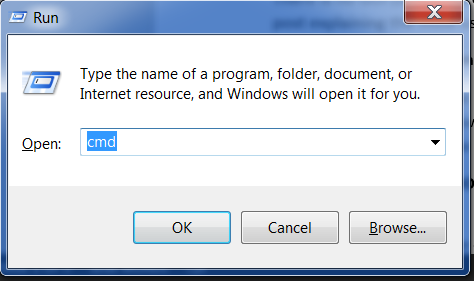
\includegraphics{unidades/unidad1/images/paste-3.png}

Más adelante en este tutorial, necesitarás tener dos consolas de
comandos abiertas a la misma vez. Sin embargo, en algunas versiones de
Windows, si ya tienes abierta una ventana de comandos e intentas abrir
otra usando el mismo método, simplemente maximizará la que ya tienes
abierta. ¡Inténtalo ahora en tu ordenador y mira qué ocurre! Si solo se
abre una ventana de comandos, intenta alguno de los otros métodos
explicados anteriormente. Al menos uno de ellos debería abrir una nueva
ventana de comandos.

\end{tcolorbox}

\begin{tcolorbox}[enhanced jigsaw, colbacktitle=quarto-callout-tip-color!10!white, colback=white, breakable, bottomrule=.15mm, opacityback=0, colframe=quarto-callout-tip-color-frame, toprule=.15mm, leftrule=.75mm, coltitle=black, bottomtitle=1mm, rightrule=.15mm, opacitybacktitle=0.6, toptitle=1mm, titlerule=0mm, left=2mm, arc=.35mm, title=\textcolor{quarto-callout-tip-color}{\faLightbulb}\hspace{0.5em}{Opening: OS X}]

Ve a Aplicaciones → Utilidades → Terminal.

\end{tcolorbox}

\chapter{Instalar Python}\label{instalar-python}

\begin{tcolorbox}[enhanced jigsaw, colbacktitle=quarto-callout-tip-color!10!white, colback=white, breakable, bottomrule=.15mm, opacityback=0, colframe=quarto-callout-tip-color-frame, toprule=.15mm, leftrule=.75mm, coltitle=black, bottomtitle=1mm, rightrule=.15mm, opacitybacktitle=0.6, toptitle=1mm, titlerule=0mm, left=2mm, arc=.35mm, title=\textcolor{quarto-callout-tip-color}{\faLightbulb}\hspace{0.5em}{Tip}]

Para lectores en casa: este capitulo se cubre en el vídeo Installing
Python \& Code Editor.

Esta sección está basada en un tutorial de Geek Girls Carrots
(https://github.com/ggcarrots/django-carrots)

\end{tcolorbox}

Django está escrito en Python. Necesitamos Python para hacer cualquier
cosa en Django. ¡Empecemos con instalarlo! Queremos que instales la
última versión de Python 3, así que si tienes una versión anterior,
necesitarás actualizarla. Si ya tienes la versión 3.4 o una superior,
debería ir bien.

Por favor, instala Python normalmente de la siguiente forma, incluso si
tienes Anaconda instalada en el ordenador.

\begin{tcolorbox}[enhanced jigsaw, colbacktitle=quarto-callout-tip-color!10!white, colback=white, breakable, bottomrule=.15mm, opacityback=0, colframe=quarto-callout-tip-color-frame, toprule=.15mm, leftrule=.75mm, coltitle=black, bottomtitle=1mm, rightrule=.15mm, opacitybacktitle=0.6, toptitle=1mm, titlerule=0mm, left=2mm, arc=.35mm, title=\textcolor{quarto-callout-tip-color}{\faLightbulb}\hspace{0.5em}{Install Python: Windows}]

Primero comprueba si tu ordenador ejecuta la versión 32 bits de Windows
o la de 64, en ``Tipo de sistema'' en la página de ``Acerca de''. Para
llegar a esta página, intenta uno de estos métodos:

\begin{itemize}
\tightlist
\item
  Presiona la tecla de Windows y la tecla Pause/Break al mismo tiempo
\item
  Abre el Panel de Control desde el menú de Windows, después accede a
  Sistema \& y Seguridad, luego a Sistema
\item
  Presiona el botón de Windows, luego accede a Configuración
  \textgreater{} Sistema \textgreater{} Acerca de
\end{itemize}

Puedes descargar Python para Windows desde la siguiente web
\url{https://www.python.org/downloads/windows/}. Clica en el enlace
``Latest Python 3 Release -Python x.x.x''. Si tu ordenador ejecuta la
versión de \textbf{64 bits} de Windows, descarga Windows x86-64
executable installer. De lo contrario, descarga \textbf{Windows x86
executable installer}. Después de descargar el instalador, deberías
ejecutarlo (dándole doble click) y seguir las instrucciones.

Una cosa para tener en cuenta: Durante la instalación, verás una ventana
de ``Setup''. Asegúrate de marcar las casillas ``Add Python 3.6 to
PATH'' o ``Add Python to your environment variables'' y hacer click en
``Install Now'', como se muestra aquí (puede que se vea un poco
diferente si estás instalando una versión diferente):

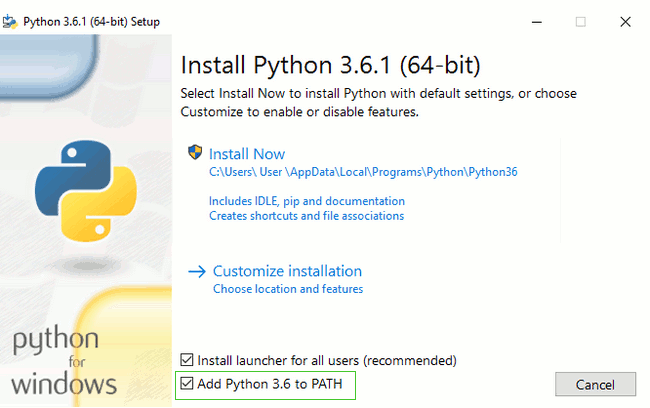
\includegraphics{unidades/unidad1/images/paste-4.png}

Cuando la instalación se complete, verás un cuadro de diálogo con un
enlace que puedes seguir para saber más sobre Python o sobre la versión
que has instalado. Cierra o cancela ese dialogo -- ¡Aprenderás más en
ese tutorial!

Nota: si estás usando una versión anterior de Windows (7, Vista o
cualquier versión anterior) y el instalador de la versión 3.6.x de
Python falla con un error, intenta también:

\begin{enumerate}
\def\labelenumi{\arabic{enumi}.}
\tightlist
\item
  instalar todas las actualizaciones de Windows e intenta instalar
  Python de nuevo; o
\item
  instalar una versión de Python anterior, por ejemplo, 3.4.6.
\end{enumerate}

Si instalas una versión anterior de Python, la pantalla de instalación
puede ser un poco diferente a la mostrada arriba. Asegúrate de
desplazarte hacia abajo para ver ``Add python.exe to Path'', después haz
click en el botón de la izquierda y selecciona ``Will be installed on
local hard drive'':

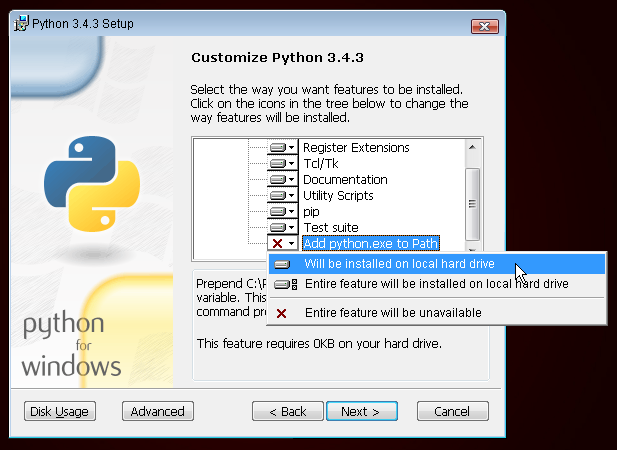
\includegraphics{unidades/unidad1/images/paste-5.png}

\end{tcolorbox}

\begin{tcolorbox}[enhanced jigsaw, colbacktitle=quarto-callout-tip-color!10!white, colback=white, breakable, bottomrule=.15mm, opacityback=0, colframe=quarto-callout-tip-color-frame, toprule=.15mm, leftrule=.75mm, coltitle=black, bottomtitle=1mm, rightrule=.15mm, opacitybacktitle=0.6, toptitle=1mm, titlerule=0mm, left=2mm, arc=.35mm, title=\textcolor{quarto-callout-tip-color}{\faLightbulb}\hspace{0.5em}{Tip}]

\textbf{Nota} Antes de instalar Python en OS X, debes asegurarte de que
la configuración del Mac permita instalar paquetes que no estén en la
App Store. ve a preferencias del sistema (System Preferences, está en la
carpeta Aplicaciones), da click en ``Seguridad y privacidad'' (Security
\& Privacy) y luego la pestaña ``General''. Si tu ``Permitir
aplicaciones descargadas desde:'' (Allow apps downloaded from:) está
establecida a ``Mac App Store,'' cambia a ``Mac App Store y
desarrolladores identificados.'' (Mac App Store and identified
developers)

Necesitas ir a la página web
https://www.python.org/downloads/release/python-361/ y descargar el
instalador de Python:

\begin{itemize}
\tightlist
\item
  Descarga el archivo Mac OS X 64-bit/32-bit installer,
\item
  Doble click en python-3.6.1-macosx10.6.pkg para ejecutar el
  instalador.
\end{itemize}

\end{tcolorbox}

\begin{tcolorbox}[enhanced jigsaw, colbacktitle=quarto-callout-tip-color!10!white, colback=white, breakable, bottomrule=.15mm, opacityback=0, colframe=quarto-callout-tip-color-frame, toprule=.15mm, leftrule=.75mm, coltitle=black, bottomtitle=1mm, rightrule=.15mm, opacitybacktitle=0.6, toptitle=1mm, titlerule=0mm, left=2mm, arc=.35mm, title=\textcolor{quarto-callout-tip-color}{\faLightbulb}\hspace{0.5em}{Install Python: Linux}]

Es muy posible que ya tengas instalado Python de serie. Para verificar
que ya lo tienes instalado (y qué versión es), abre una consola y
escribe el siguiente comando:

\begin{Shaded}
\begin{Highlighting}[]
\ExtensionTok{$}\NormalTok{ python3 }\AttributeTok{{-}{-}version}
\ExtensionTok{Python}\NormalTok{ 3.6.1}
\end{Highlighting}
\end{Shaded}

Si tienes instalada una versión diferente de Python, al menos 3.4.0 (por
ejemplo 3.6.0), entonces no tienes que actualizar. Si tu no has
instalado Python, o si tu quieres una versión diferente, primero
verifica que distribución de Linux estás usando con el siguiente
comando:

\begin{Shaded}
\begin{Highlighting}[]
\ExtensionTok{$}\NormalTok{ grep \^{}NOMBRE= /etc/os{-}release}
\end{Highlighting}
\end{Shaded}

Después, dependiendo de el resultado, sigue una de las siguientes guías
de instalación bajo ésta sección.

\end{tcolorbox}

\begin{tcolorbox}[enhanced jigsaw, colbacktitle=quarto-callout-tip-color!10!white, colback=white, breakable, bottomrule=.15mm, opacityback=0, colframe=quarto-callout-tip-color-frame, toprule=.15mm, leftrule=.75mm, coltitle=black, bottomtitle=1mm, rightrule=.15mm, opacitybacktitle=0.6, toptitle=1mm, titlerule=0mm, left=2mm, arc=.35mm, title=\textcolor{quarto-callout-tip-color}{\faLightbulb}\hspace{0.5em}{Install Python: Debian or Ubuntu}]

Escribe este comando en tu consola:

\begin{Shaded}
\begin{Highlighting}[]
\ExtensionTok{$}\NormalTok{ sudo apt install python3}
\end{Highlighting}
\end{Shaded}

\end{tcolorbox}

\begin{tcolorbox}[enhanced jigsaw, colbacktitle=quarto-callout-tip-color!10!white, colback=white, breakable, bottomrule=.15mm, opacityback=0, colframe=quarto-callout-tip-color-frame, toprule=.15mm, leftrule=.75mm, coltitle=black, bottomtitle=1mm, rightrule=.15mm, opacitybacktitle=0.6, toptitle=1mm, titlerule=0mm, left=2mm, arc=.35mm, title=\textcolor{quarto-callout-tip-color}{\faLightbulb}\hspace{0.5em}{Tip}]

Install Python: Fedora

Usa este comando en tu consola:

\begin{Shaded}
\begin{Highlighting}[]
\ExtensionTok{$}\NormalTok{ sudo dnf install python3}
\end{Highlighting}
\end{Shaded}

Si estás en versiones antiguas de Fedora, puedes obtener un error que el
comando dnf no se encuentra. En ese caso, necesitas usar yum en su
lugar.

\end{tcolorbox}

\begin{tcolorbox}[enhanced jigsaw, colbacktitle=quarto-callout-tip-color!10!white, colback=white, breakable, bottomrule=.15mm, opacityback=0, colframe=quarto-callout-tip-color-frame, toprule=.15mm, leftrule=.75mm, coltitle=black, bottomtitle=1mm, rightrule=.15mm, opacitybacktitle=0.6, toptitle=1mm, titlerule=0mm, left=2mm, arc=.35mm, title=\textcolor{quarto-callout-tip-color}{\faLightbulb}\hspace{0.5em}{Tip}]

Install Python: openSUSE

Usa este comando en tu consola:

\begin{Shaded}
\begin{Highlighting}[]
\ExtensionTok{$}\NormalTok{ sudo zypper install python3}
\end{Highlighting}
\end{Shaded}

\end{tcolorbox}

Verifica si la instalación fue exitosa abriendo una terminal o consola,
y corriendo el comando python3:

\begin{Shaded}
\begin{Highlighting}[]
\ExtensionTok{$}\NormalTok{ python3 }\AttributeTok{{-}{-}version}
\ExtensionTok{Python}\NormalTok{ 3.6.1}
\end{Highlighting}
\end{Shaded}

La versión mostrada puede ser diferente desde 3.6.1 -- debería marcar la
versión que instalaste.

\textbf{NOTA:} Si está en Windows y recibe un mensaje de error que
indica que python3 no se encontró, intente usar python (sin el 3) y
compruebe si todavía podría ser una versión de Python que sea 3.4.0 o
superior. Si eso tampoco funciona, puede abrir un nuevo símbolo del
sistema e intentar nuevamente; Esto sucede si usa un símbolo del sistema
abierto antes de la instalación de Python.

Si tienes alguna duda, o si ocurrió algún error y no tienes idea sobre
qué hacer, ¡por favor pregunta a tu entrenador! Algunas veces las cosas
no van bien y es mejor pedir ayuda a alguien con más experiencia.

Instala un Editor de Código

Hay muchos editores diferentes y la elección es principalmente una
cuestión de preferencia personal. La mayoría de programadores de Python
usan IDEs (Entornos de Desarrollo Integrados) complejos pero muy
potentes, como PyCharm. Sin embargo, como principiante, probablemente no
es lo más aconsejable; nuestras recomendaciones son igualmente potentes
pero mucho más simples.

Abajo presentamos nuestras sugerencias pero también puedes preguntarle a
tu mentora cuáles son las suyas -será más fácil que te ayude.

\chapter{Visual Studio Code}\label{visual-studio-code}

Visual Studio Code es un recurso de edición de código desarrollado por
Microsoft para Windows, Linux y macOS. Esto incluye soporte para
depuración, control de Git incrustado, sintaxis destacada, completación
de código inteligente, fragmentos y refactorización de código.

\href{https://code.visualstudio.com/download}{Descárgalo aquí}

\chapter{Gedit}\label{gedit}

Gedit es un editor gratuito de código abierto, disponible para todos los
sistemas operativos.

\href{https://gedit-technology.github.io/apps/gedit/}{Descárgalo aquí}

\chapter{Sublime Text}\label{sublime-text}

Sublime Text es un editor muy popular con un periodo de prueba gratis, y
está disponible para todos los sistemas operativos.

\href{https://www.sublimetext.com/}{Descárgalo aquí}

\chapter{¿Por qué estamos instalando un editor de
código?}\label{por-quuxe9-estamos-instalando-un-editor-de-cuxf3digo}

Tú podrías estar preguntándote por qué estamos instalando este
especializado software editor de código en vez de usar algo como Word o
Notepad.

La primera razón es que el código necesita ser texto plano, y el
problema con programas como Word y Textedit es que no producen texto
plano, sino texto enriquecido (con fuentes y formatos), usando formatos
personalizados como
\href{https://en.wikipedia.org/wiki/Rich_Text_Format}{RTF ( Formato del
Texto Enriquecido, del inglés Rich Text Format)}.

La segunda razón es que los editores de código están especializados para
esta función, así ellos pueden proveer ayuda a características como
destacar código con color acorde a su significado, o automáticamente
cerrando etiquetas para ti.

Veremos todo esto en acción más adelante. Pronto pensarás en convertir
el editor de código en una de tus herramientas favoritas. :)

\chapter{Configura el entorno virtual (virtualenv) e instala
Django}\label{configura-el-entorno-virtual-virtualenv-e-instala-django}

Parte de esta sección está basada en tutoriales por Geek Girls Carrots
(\url{https://github.com/ggcarrots/django-carrots}).

Parte de este capítulo está basada en el django-marcador tutorial bajo
la licencia Creative Commons Attribution-ShareAlike 4.0 internacional.
El tutorial de django-marcador tiene derechos de autor de Markus
Zapke-Gündemann et al.

\chapter{Entorno virtual}\label{entorno-virtual-1}

Antes de instalar Django, instalaremos una herramienta extremadamente
útil que ayudará a mantener tu entorno de desarrollo ordenado en tu
computadora. Es posible saltarse este paso, pero es altamente
recomendable. ¡Empezar con la mejor configuración posible te ahorrará
muchos problemas en el futuro!

Así que, vamos a crear un entorno virtual (también llamado un
virtualenv). Virtualenv aísla tu configuración de Python/Django para
cada proyecto. Esto quiere decir que cualquier cambio que hagas en un
sitio web no afectará a ningún otro que estés desarrollando. Genial,
¿no?

Todo lo que necesitas hacer es encontrar un directorio en el que quieras
crear el virtualenv; tu directorio home, por ejemplo. En Windows, puede
verse como \textbf{C : ~Users ~Name} (donde Name es el nombre de tu
usuario).

\begin{tcolorbox}[enhanced jigsaw, colbacktitle=quarto-callout-tip-color!10!white, colback=white, breakable, bottomrule=.15mm, opacityback=0, colframe=quarto-callout-tip-color-frame, toprule=.15mm, leftrule=.75mm, coltitle=black, bottomtitle=1mm, rightrule=.15mm, opacitybacktitle=0.6, toptitle=1mm, titlerule=0mm, left=2mm, arc=.35mm, title=\textcolor{quarto-callout-tip-color}{\faLightbulb}\hspace{0.5em}{Tip}]

\textbf{NOTA:} En Windows, asegúrate de que este directorio no contiene
caracteres especiales o acentuados; si tu nombre de usuario contiene
caracteres acentuados, usa un directorio distinto, por ejemplo
C:\djangogirls.

\end{tcolorbox}

Para este tutorial usaremos un nuevo directorio djangogirls en tu
directorio home:

\begin{Shaded}
\begin{Highlighting}[]
\ExtensionTok{$}\NormalTok{ mkdir djangogirls}
\ExtensionTok{$}\NormalTok{ cd djangogirls}
\end{Highlighting}
\end{Shaded}

Haremos un virtualenv llamado myvenv. El comando general estará en el
formato:

\begin{Shaded}
\begin{Highlighting}[]
\ExtensionTok{$}\NormalTok{ python3 }\AttributeTok{{-}m}\NormalTok{ venv myvenv}
\end{Highlighting}
\end{Shaded}

\begin{tcolorbox}[enhanced jigsaw, colbacktitle=quarto-callout-tip-color!10!white, colback=white, breakable, bottomrule=.15mm, opacityback=0, colframe=quarto-callout-tip-color-frame, toprule=.15mm, leftrule=.75mm, coltitle=black, bottomtitle=1mm, rightrule=.15mm, opacitybacktitle=0.6, toptitle=1mm, titlerule=0mm, left=2mm, arc=.35mm, title=\textcolor{quarto-callout-tip-color}{\faLightbulb}\hspace{0.5em}{Virtual environment: Windows}]

Para crear un nuevo virtualenv, necesitas abrir una terminal ``command
prompt'' y ejecutar python -m venv myvenv. Se verá así:

\begin{Shaded}
\begin{Highlighting}[]
\ExtensionTok{C:\textbackslash{}Users\textbackslash{}Name\textbackslash{}djangogirls}\OperatorTok{\textgreater{}}\NormalTok{ python }\AttributeTok{{-}m}\NormalTok{ venv myvenv}
\end{Highlighting}
\end{Shaded}

Donde myvenv es el nombre de tu virtualenv. Puedes utilizar cualquier
otro nombre, pero asegúrate de usar minúsculas y no usar espacios,
acentos o caracteres especiales. También es una buena idea mantener el
nombre corto. ¡Vas utilizarlo muchas vecesl!

\end{tcolorbox}

\begin{tcolorbox}[enhanced jigsaw, colbacktitle=quarto-callout-tip-color!10!white, colback=white, breakable, bottomrule=.15mm, opacityback=0, colframe=quarto-callout-tip-color-frame, toprule=.15mm, leftrule=.75mm, coltitle=black, bottomtitle=1mm, rightrule=.15mm, opacitybacktitle=0.6, toptitle=1mm, titlerule=0mm, left=2mm, arc=.35mm, title=\textcolor{quarto-callout-tip-color}{\faLightbulb}\hspace{0.5em}{Virtual environment: Linux and OS X}]

Podemos crear un virtualenv en Linux y OS X, es tan sencillo como
ejecutar python3 -m venv myvenv. Se verá así:

\begin{Shaded}
\begin{Highlighting}[]
\ExtensionTok{$}\NormalTok{ python3 }\AttributeTok{{-}m}\NormalTok{ venv myvenv}
\end{Highlighting}
\end{Shaded}

myvenv es el nombre de tu virtualenv. Puedes usar cualquier otro nombre,
pero sólo utiliza minúsculas y no incluyas espacios. También es una
buena idea mantener el nombre corto. ¡Vas a referirte muchas veces a él!

\begin{tcolorbox}[enhanced jigsaw, colbacktitle=quarto-callout-tip-color!10!white, colback=white, breakable, bottomrule=.15mm, opacityback=0, colframe=quarto-callout-tip-color-frame, toprule=.15mm, leftrule=.75mm, coltitle=black, bottomtitle=1mm, rightrule=.15mm, opacitybacktitle=0.6, toptitle=1mm, titlerule=0mm, left=2mm, arc=.35mm, title=\textcolor{quarto-callout-tip-color}{\faLightbulb}\hspace{0.5em}{Tip}]

\begin{verbatim}
**NOTA:** En algunas versiones de Debian/Ubuntu, puede que obtengas el siguiente error:

``` bash

The virtual environment was not created successfully because ensurepip is not available.  En sistemas Debian/Ubuntu, tendrás que instalar el paquete python3-venv usando el siguiente comando.
   apt-get install python3-venv
Puede que tengas que usar sudo con este comando.  Después de instalar el paquete python3-venv, vuelve a crear tu entorno virtual.
```

En este caso, sigue las instrucciones anteriores e instala el paquete python3-venv:

``` bash
$ sudo apt install python3-venv
```
NOTA: En algunas versiones de Debian/Ubuntu inicializar el entorno virtual de esta manera da el siguiente error:

``` bash
Error: Command '['/home/eddie/Slask/tmp/venv/bin/python3', '-Im', 'ensurepip', '--upgrade', '--default-pip']' returned non-zero exit status 1
```

Para evitar esto, utiliza directamente el comando virtualenv.

``` bash
$ sudo apt-get install python-virtualenv
$ virtualenv --python=python3.6 myvenv
```
NOTA: Si obtienes un error como

``` bash
E: Unable to locate package python3-venv
```
entonces ejecuta:

``` bash
sudo apt install python3.6-venv
```
\end{verbatim}

\end{tcolorbox}

\end{tcolorbox}

\chapter{Trabajar con virtualenv}\label{trabajar-con-virtualenv}

El comando anterior creará un directorio llamado myvenv (o cualquier
nombre que hayas elegido) que contiene nuestro entorno virtual
(básicamente un montón de archivos y carpetas).




\end{document}
